\documentclass{sig-alternate}

\begin{document}
\conferenceinfo{OZCHI}{'14, Dec 2-5, 2014, Sydney, Australia}

\title{Visualising a Live Coding Arts Process}

\numberofauthors{3} 
\author{
\alignauthor Anon1\\
       \affaddr{-}\\
       \affaddr{-}\\
       \email{-}
\alignauthor Anon2\\
       \affaddr{-}\\
       \affaddr{-}\\
       \email{-}
\alignauthor Anon3\\
       \affaddr{-}\\
       \affaddr{-}\\
       \email{-}
}

\maketitle
\begin{abstract}

We have investigated software visualisations as a means to communicate the programming process of ``live coding'' computer music performances. Following a field study at a festival of the contemporary arts, two sets of complementary, interaction-driven ``aesthetic" and ``didactic" visualisations were incorporated into a live coding system. A formal audience experiment was undertaken to evaluate the visualisations' contributions to the audience experience, with emphasis on two (self-reported) experiential dimensions of  ``understanding'' and ``enjoyment''. The reactions of the live coding performer (the programmer) were also evaluated in a video-cued-recall interview.

A majority of the audience in the formal experiment reported that both sets of software visualisations enhanced their ``enjoyment". Reported audience ``understanding" was more problematic. Although more of the audience reported that the ``didactic" (rather than the ``aesthetic") visualisations helped them to ``understand" the process, the reported levels of ``understanding" fluctuated during the course of the performances in a way that did not seem to preference one visualisation type over the other. Evaluation of the reactions of the live coder were notably different to that of the audience. This observation, and our study overall, motivate an ongoing challenge to develop live coding visualisations which better align the mental models of performer and audience to enhance the experiences of all.

\end{abstract}

\category{H.5}{Information Interfaces and Presentation}{Miscellaneous}

\terms{Experimentation, Design}

\keywords{Live coding, software visualisation}

\section{Introduction}

``Show us your screens... Code should be seen as well as heard'', says the draft manifesto of the international organisation ``TOPLAP'' \cite{Toplap} which is devoted to the decade-old arts performance practice ``live coding''. Live coding is a performance practice where computer code is created in front of a live audience to generate computer music, video and visualisations in real time. The ``show us your screens'' exhortation underscores the need for authenticity to distinguish this artform from aligned performance art genres such as VJ'ing. 

Live computer music is the primary product of live coding. Where they exist, live coded graphics and video are launched and orchestrated directly by commands from the computer keyboard for artistic impact. Commonly, non-expert live coding audience members spend much of their time staring at raw computer code (text-based or visual programming languages) and, until now, no formal study has ever been undertaken to gauge an audience's understanding of that computer code and whether, from an audience perspective, code really should be ``seen as well as heard''.

Traditional approaches to visualising code focus on historic source code changes, the behaviour of algorithms or the structure of the source code rather than the \textit{process of programming} (see \cite{Novais2013}). Furthermore, within the space of artistic live coding most of the academic treatment of visualisations have adopted a design or survey approach \cite{McLean2010b,Magnusson2013} and have not subjected alternatives to rigorous evaluation.

In this paper, we set out to evaluate the audience reception to the display of code during live coding performances and to see whether code-driven visualisations might improve both the audience enjoyment and the audience understanding of these performances.

\section{Field Study}

On one evening of the (name withheld for blind reviewing) arts festival in (withheld), a survey was presented to the audience of a live coding computer music performance. The survey was designed to gain an impression of the audience's response to the performance and to the projection of the computer code (a Scheme based language with syntax highlighting). Alongside demographic and open-ended questions, audience members were solicited to indicate which of a number of curves best represented their personal ``enjoyment'' and ``understanding'' of the performer's actions in typing the computer code through the performance. These curves were analysed based on their binning into ``high", ``medium", and ``low'' categories for the ``beginning'', ``middle'' and ``end'' of the performance. Other survey questions addressed the sense of ``liveness'' of the performance \cite{Auslander} and whether the code-projections were found to be confusing.

Of the 13 survey responses received, 6 indicated a high level of enjoyment throughout the whole performance with the remaining 7 responses mostly indicating alternating levels of enjoyment. No responses indicated a low level of enjoyment throughout the performance.

Only 2 of the 13 respondents indicated that they understood the relationship between the code projections and the music throughout the performance. Although a Chi-square analysis revealed no significant relationship between ``enjoyment'' and ``understanding'' per se, it was remarkable that 3 of the 6 respondents who indicated a high level of ``enjoyment" throughout the performance, also indicated a pattern of ``understanding" that increased from low to high as the performance progressed. Nine of the 13 respondents stated that the code projections provided a sense of liveness to the performance and the remainder stated that viewing the code had no effect on their sense of liveness. Four respondents felt that the code projections were confusing, 5 stated that they were not, and 4 did not answer the question.

Taken as a whole, the results of this small field study were salutatory for the notion of ``seeing as well as hearing'' code during a live coding performance, especially as far as the general public is concerned. The best that can be said for the code projections is that a majority of the audience felt that they made the performance seem more ``live''. However a minority stated that they found the projections confusing and only a very small number of respondents claimed to have actually understood what the programmer was doing. We were quite intrigued by the small cohort of respondents whose understanding increased through the performance and whose enjoyment remained high, and we wished to test whether augmenting code projections with additional visualisations might increase this pattern of understanding, and enjoyment across an audience. 

\section{Design}

\begin{figure}
\centering
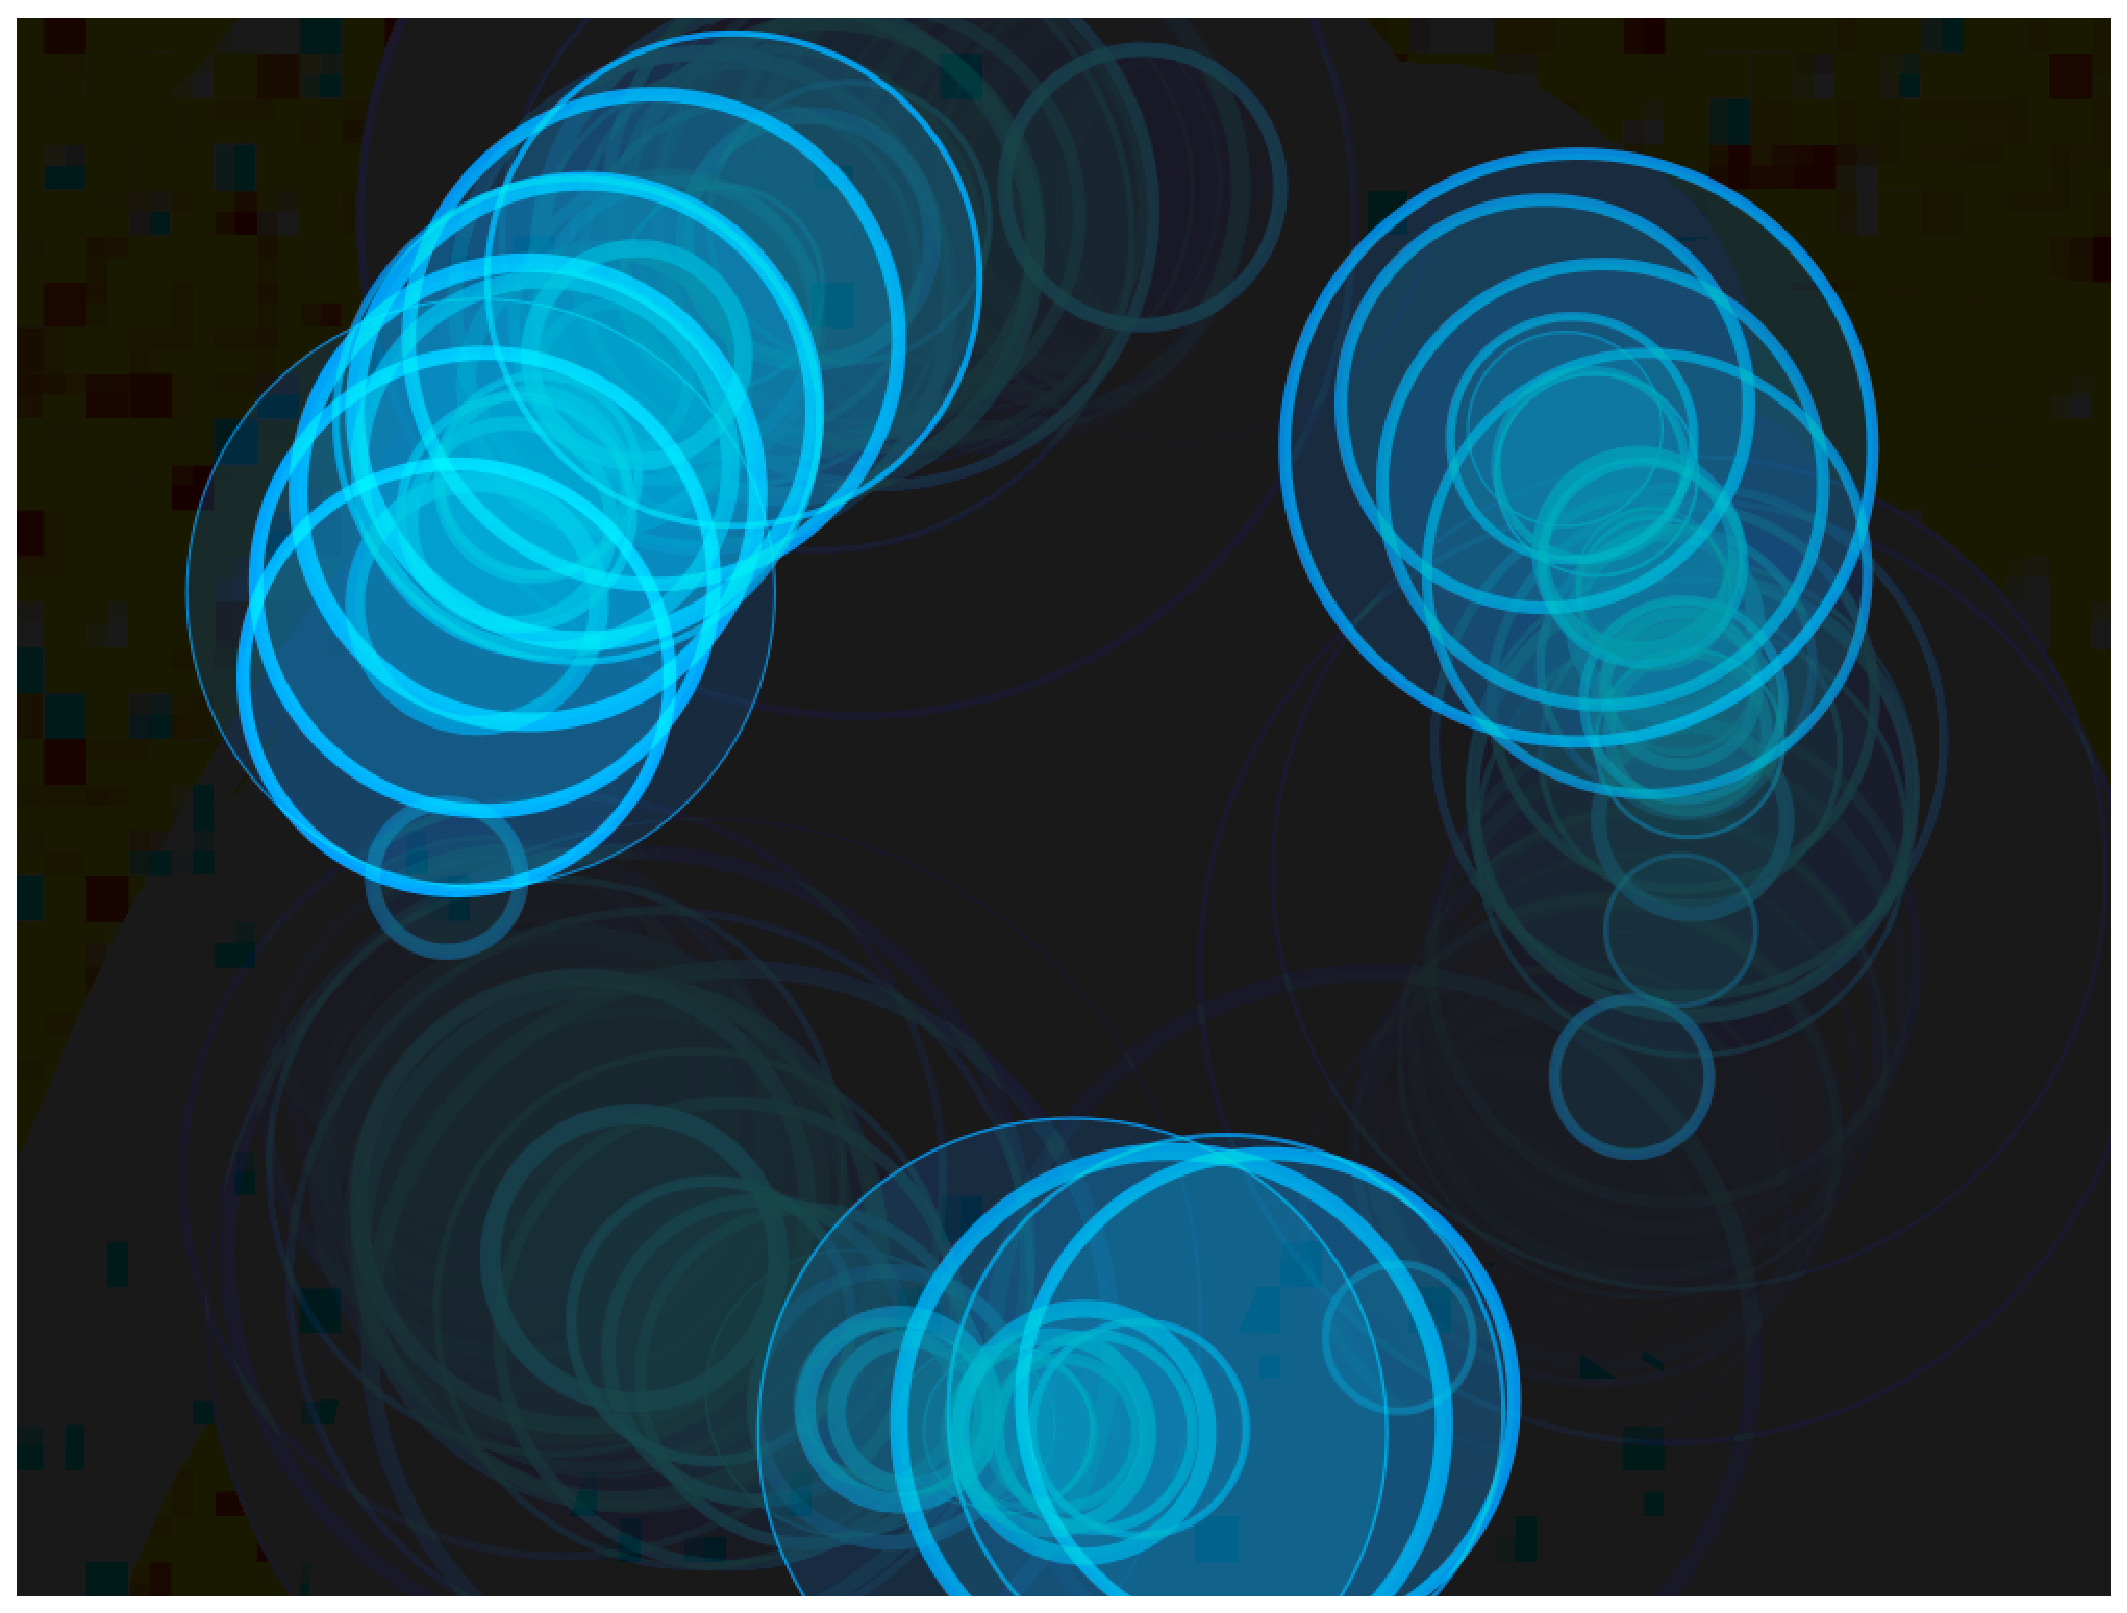
\epsfig{file=aesthetic-vis.eps, width=3.4in}
\caption{Example aesthetic visualisation. This and all subsequent figures are \textit{best viewed in colour}.}
\label{fig:aesthetic-visualisation}
\end{figure}

\begin{figure}
\centering
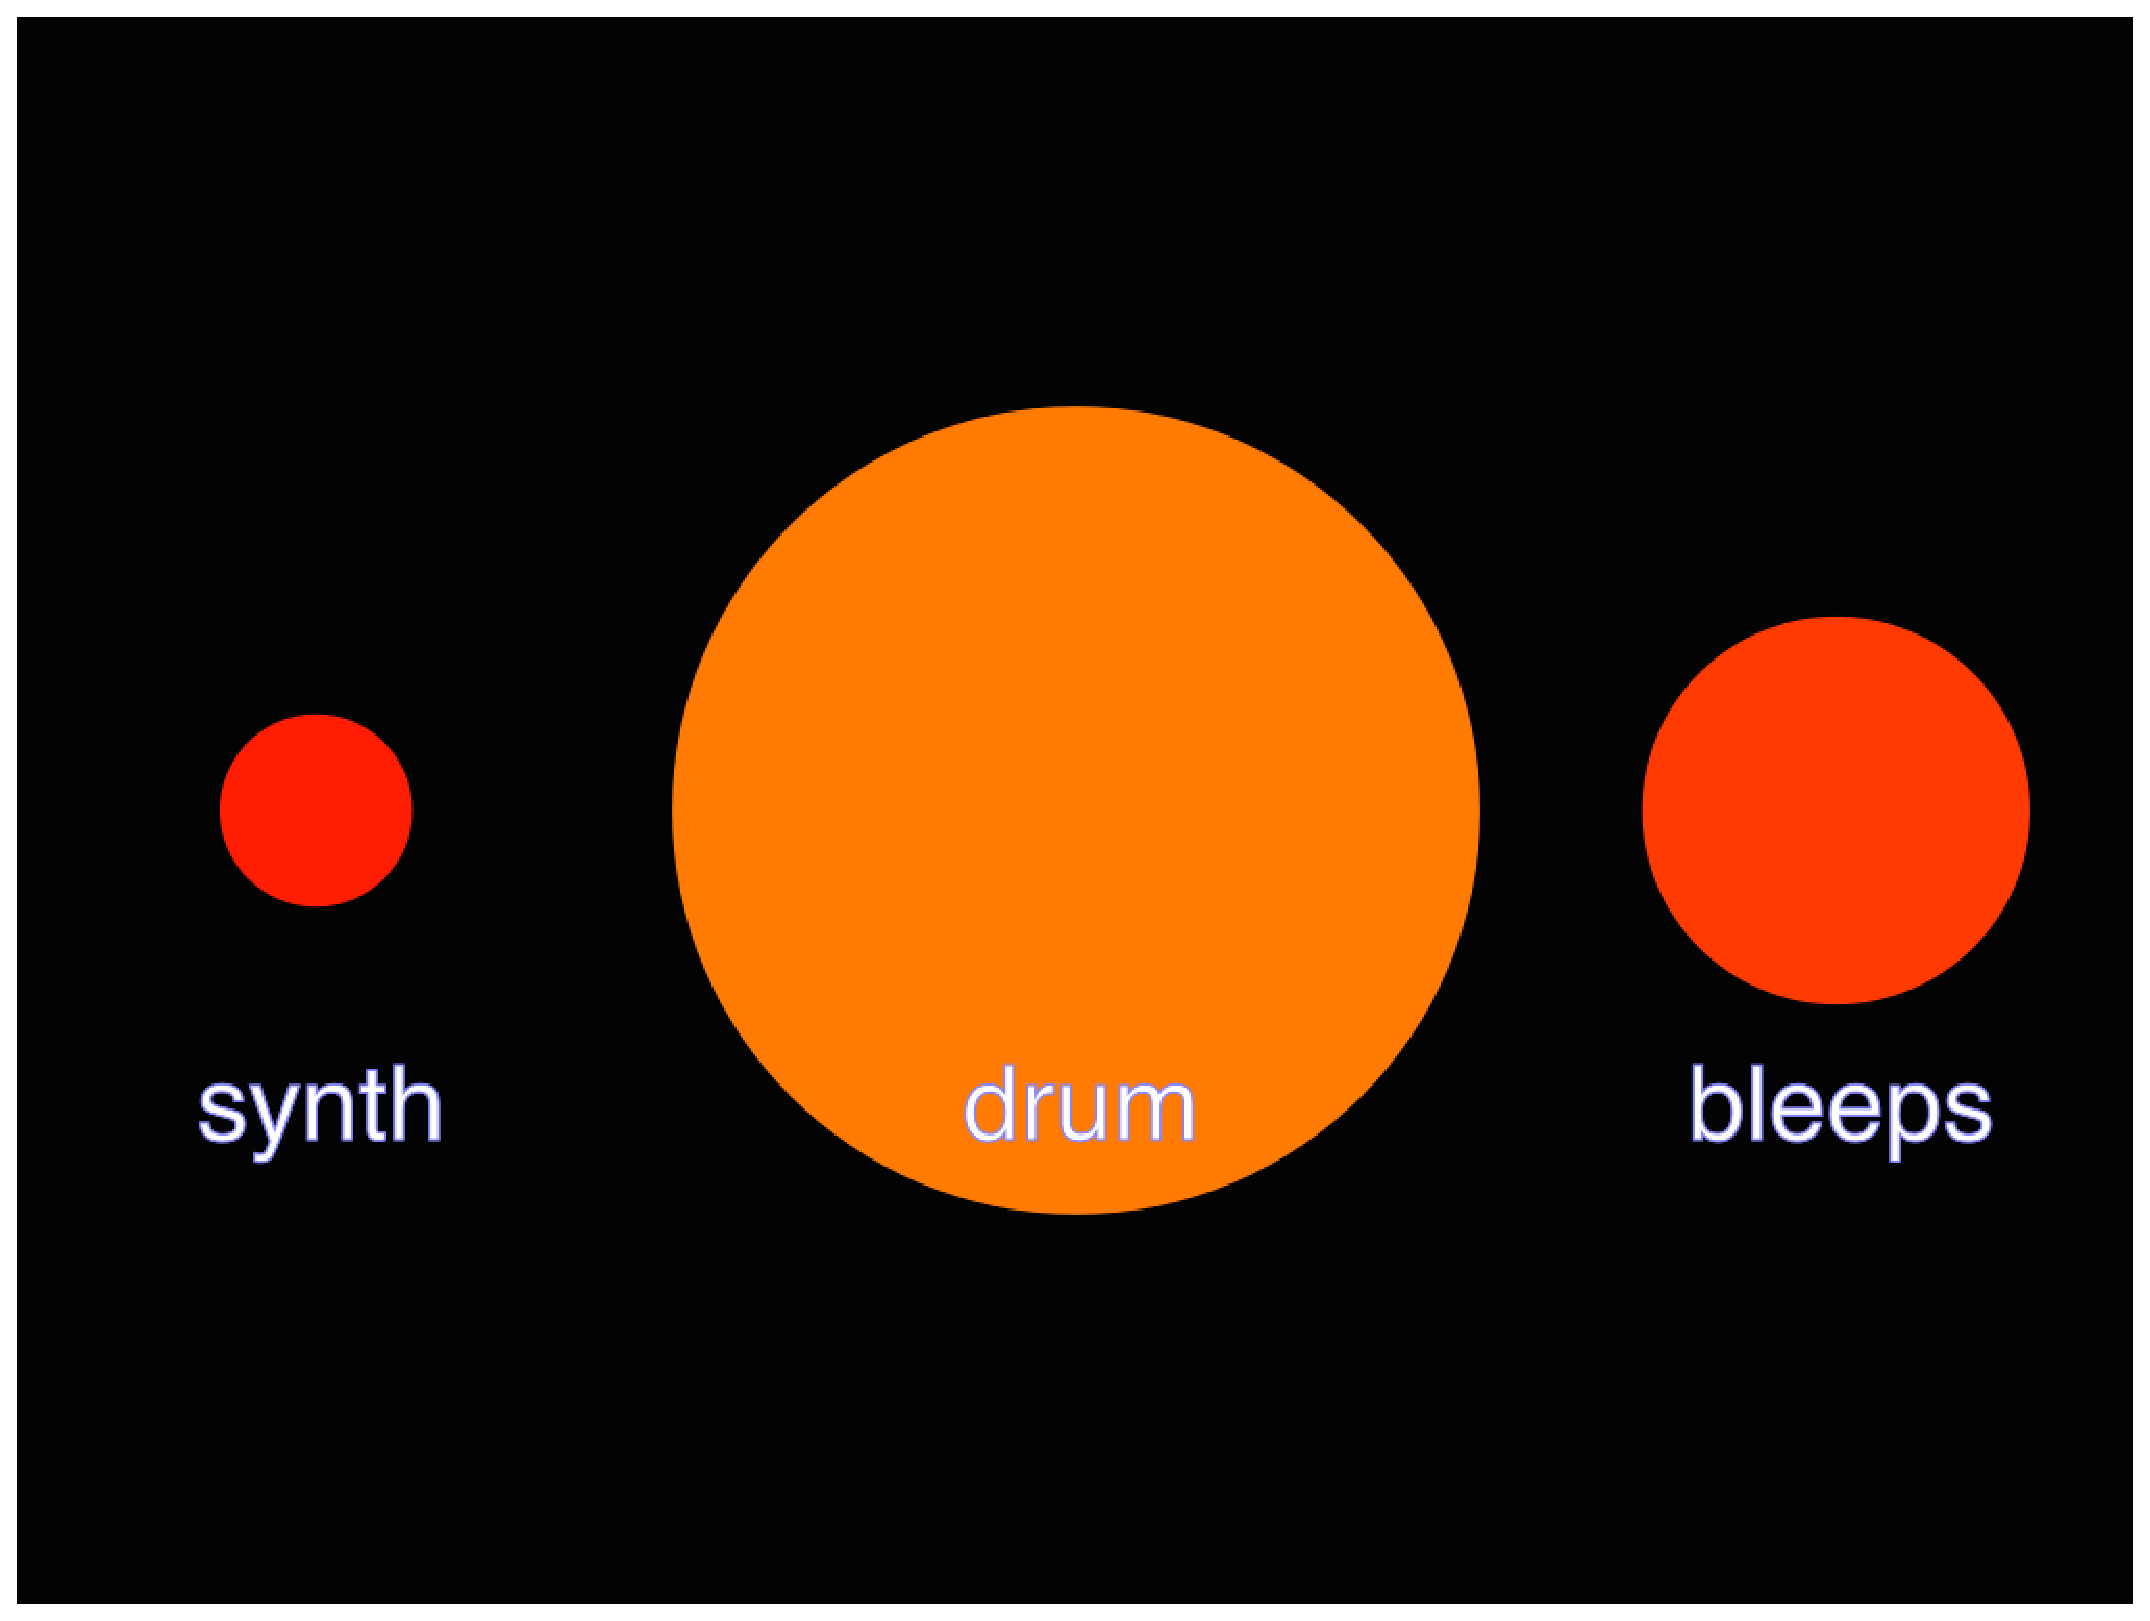
\epsfig{file=didactic-vis.eps, width=3.4in}
\caption{Example didactic visualisation.}
\label{fig:didactic-visualisation}
\end{figure}

Two sets of visualisations were developed based on the results of the initial survey and the literature. The first set focussed on increasing audience retention and user experience by maximising aesthetic appeal \cite{Cawthon2007} while communicating the actions of the programmer. The second set attempted to communicate program behaviour and visualise output while communicating the actions of the programmer. These two approaches will be referred to as the ``aesthetic'' condition and the ``didactic'' condition respectively.

The set of ``aesthetic'' visualisations focussed less on the programmatic aspects of the live coding performance, rather intending to provide additional visual interest to the projected code thereby prolonging attention. More variety was used in visual structure and colour. Again, four visualisations were presented, varying the visualisation based on the number of active functions. It was predicted that focussing on the aesthetic nature of the visualisations would assist in audience retention and result in a consistency of interest through the performance.

The set of ``didactic'' visualisations predominantly focussed on the relationship between the live coding active processes and their behaviour. The visualisations prominently displaying the names of the active functions with visual indication of the number of functions running and their callback time. Bright colours and solid shapes were used to ensure constant visibility and communicate the intention of the underlying code. Overall, four visualisations were presented with each introduced depending on the number of active functions. It was predicted that taking a more educational approach would see a reduction in audience confusion through the performance.

% Henry's edit below.

% Two sets of visualisations were developed based on the results of the initial survey and the literature. A set of ``aesthetic" visualisations focussed on enhancing the audience experience by rendering attractive and engaging graphics which spawned and moved in time with the keyboard presses (?TRUE? OR THE MUSIC ITSELF?) of the performer. 
% The second set of visualisations attempted to communicate the actions of the programmer and the main software components that were created and modified by the programmer over time. 

% The ``didactic" visualisations predominantly focussed on the relationship between the active software processes and their behaviour. They prominently displaying the {\it names} of the active functions together with indications of the number of functions running and their callback times. Bright colours and solid shapes were used to ensure constant visibility and to communicate the intention of the underlying code. Overall, up-to four visualisations were presented with each introduced depending on the number of active functions. It was hypothesised that taking a didactic approach to visualising the live-coding process would result in enhanced audience ``understanding", and a reduction in audience ``confusion", through the performance.

% The set of ``aesthetic" visualisations (\cite{Cawthon2007} (ALSO CITE MClEAN?) (HOW EXACTLY DID YOU MAXIMISE AESTHETIC APPEAL? HOW WERE THE AESTHETIC VISUALISATIONS DIVEN? WERE THEY IN SYNCH WITH THE METRONOME?)focussed less on the programmatic aspects of the live coding performance, rather intending to provide additional visual interest to the performance and thereby prolonging attention. Compared with the ``didactic" set, more variety was used in visual structure and colour. Once again, four visualisations were presented, varying the visualisation based on the number of active software functions, but these visualisations were unlabelled and they moved and interacted with each other over the entire projected scene.(TRUE?) It was predicted that focussing on the aesthetic nature of the visualisations would assist in audience retention and result in a consistency of interest through the performance.

\section{User Study}

Our visualisations were presented to the audiences of two live coding performances. Each performance was run as two, ten-minute, improvised computer music pieces with each piece demonstrating one of the two visualisation types. The experiment was run twice, with non-overlapping audience members. The order of presentations of the visualisation types was swapped between performances. Audience members were recruited on the basis of being treated to a computer music performance. In our experimental design we considered, but decided against, the inclusion of a third condition of ``code with no visualisation'' on the basis of the resulting experimental design making it difficult to recruit audience participants and causing audience and performer fatigue (particularly when taking order-balancing into consideration). 

Over the course of each performance, the audience members completed a survey consisting of four sections. These included demographic information, their opinion of the first piece, their opinion of the second piece and some overall questions. Questions regarding each piece predominantly focussed on reporting levels of ``enjoyment" and ``understanding" related to the visualisation while the final section focussed on eliciting potential improvements.
% The experiment and survey design were endorsed by Ethics Protocol (details omitted for blind review).

Subsequent to the audience experiment a video-cued-recall interview was conducted with the live coder. One performance was examined critically and comparisons were drawn between the live coder's statements and the results of the audience surveys.

\subsection{Results}

A total of 41 audience survey responses were received with a split of 19 and 22 participants in each of the performances. Of this survey population, $66\%$ were male, $76\%$ were aged between 18 and 32 and $78\%$ of the participants had never seen a live coding performance before.

Audience ``enjoyment" and ``understanding" were evaluated for the two sets of visualisations as described below. A significance level of $0.05$ was used with a chi-squared analysis.

\subsubsection{``Enjoyment''}

\begin{figure}
\centering
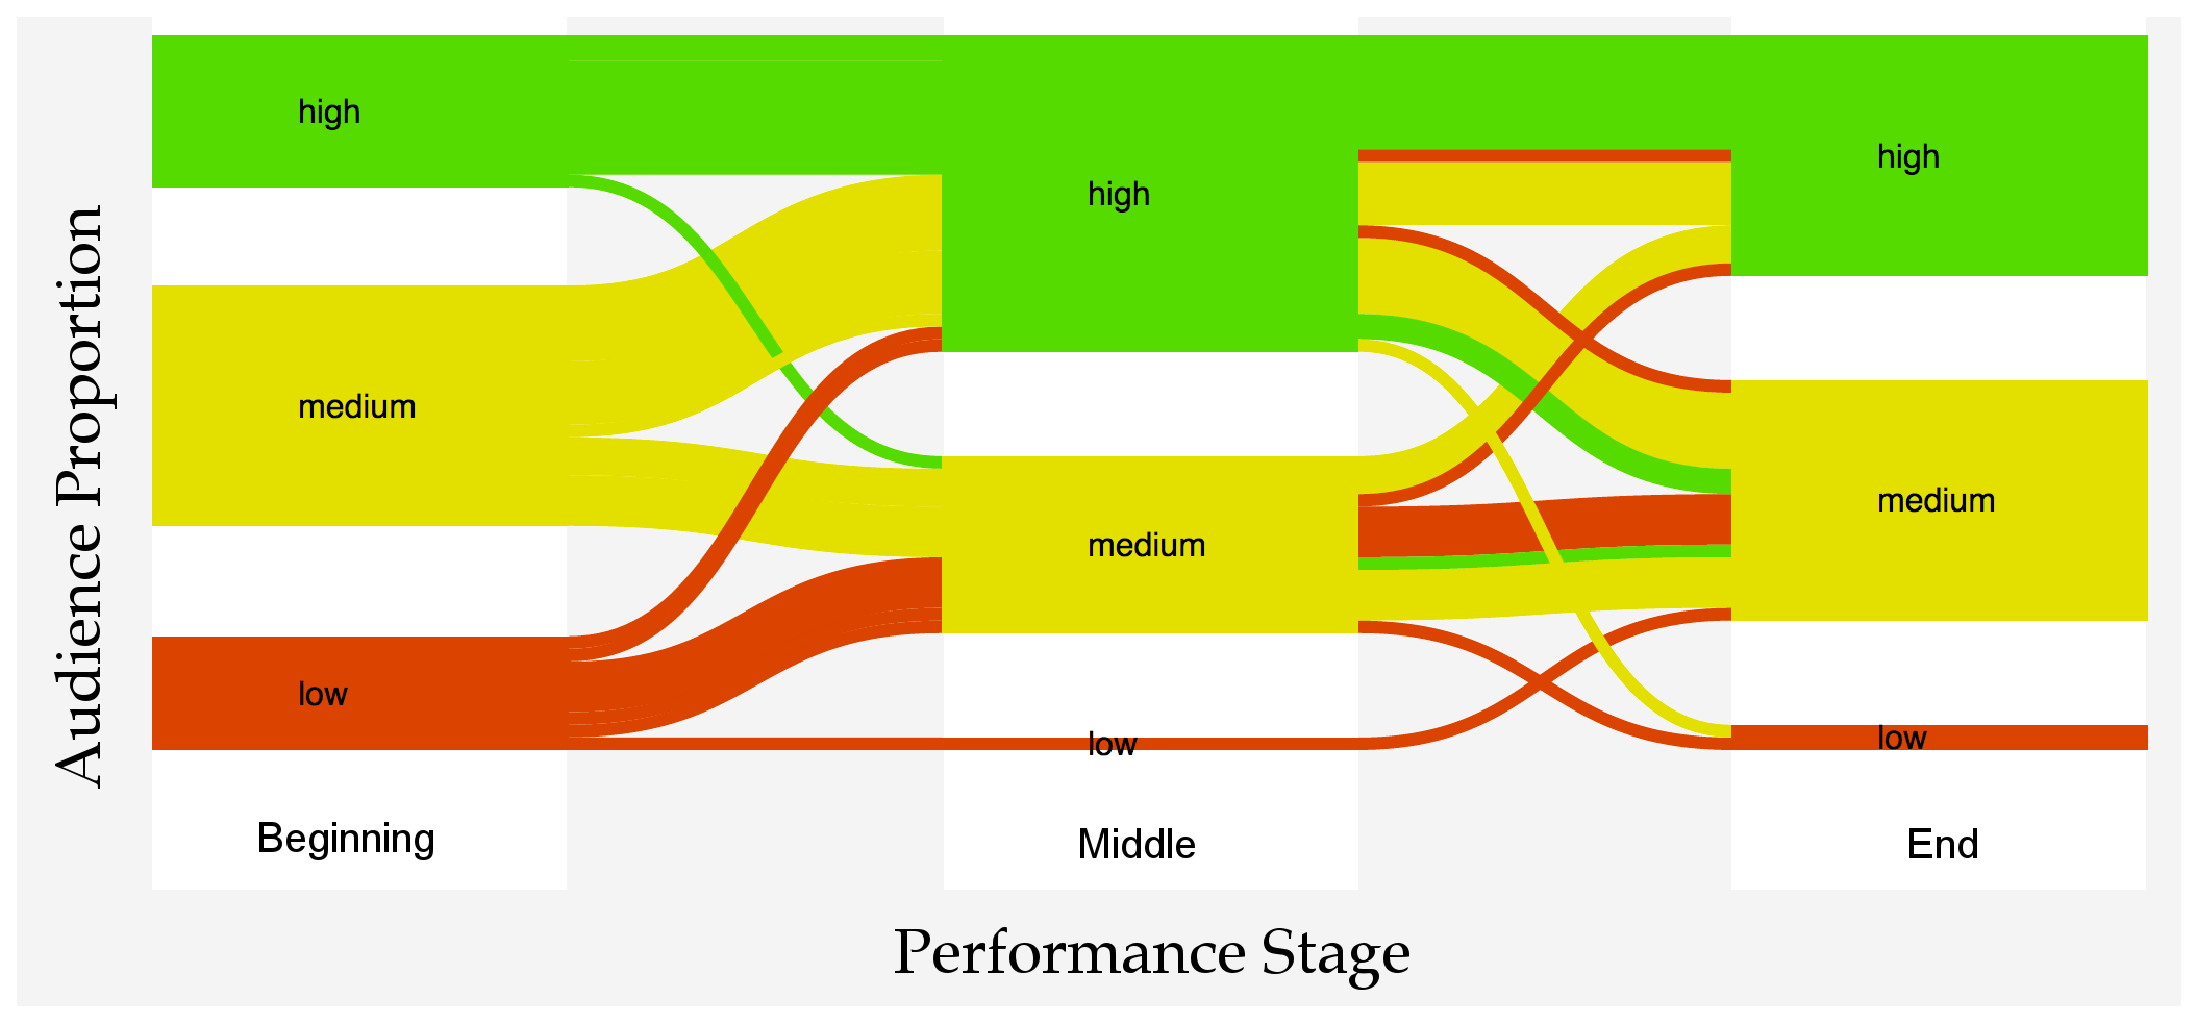
\epsfig{file=aesthetic-enjoyment-final.eps, width=3.4in}
\caption{Audience reported enjoyment level during the beginning, middle and end of the performance with the ``aesthetic'' condition. For this and all subsequent graphs of this type, line width indicates proportion of the audience reporting high, medium or low and link colour between the three performance stages indicates the reported level at the \textit{beginning} of the performance.}
\label{fig:aesthetic-enjoyment}
\end{figure}

\begin{figure}
\centering
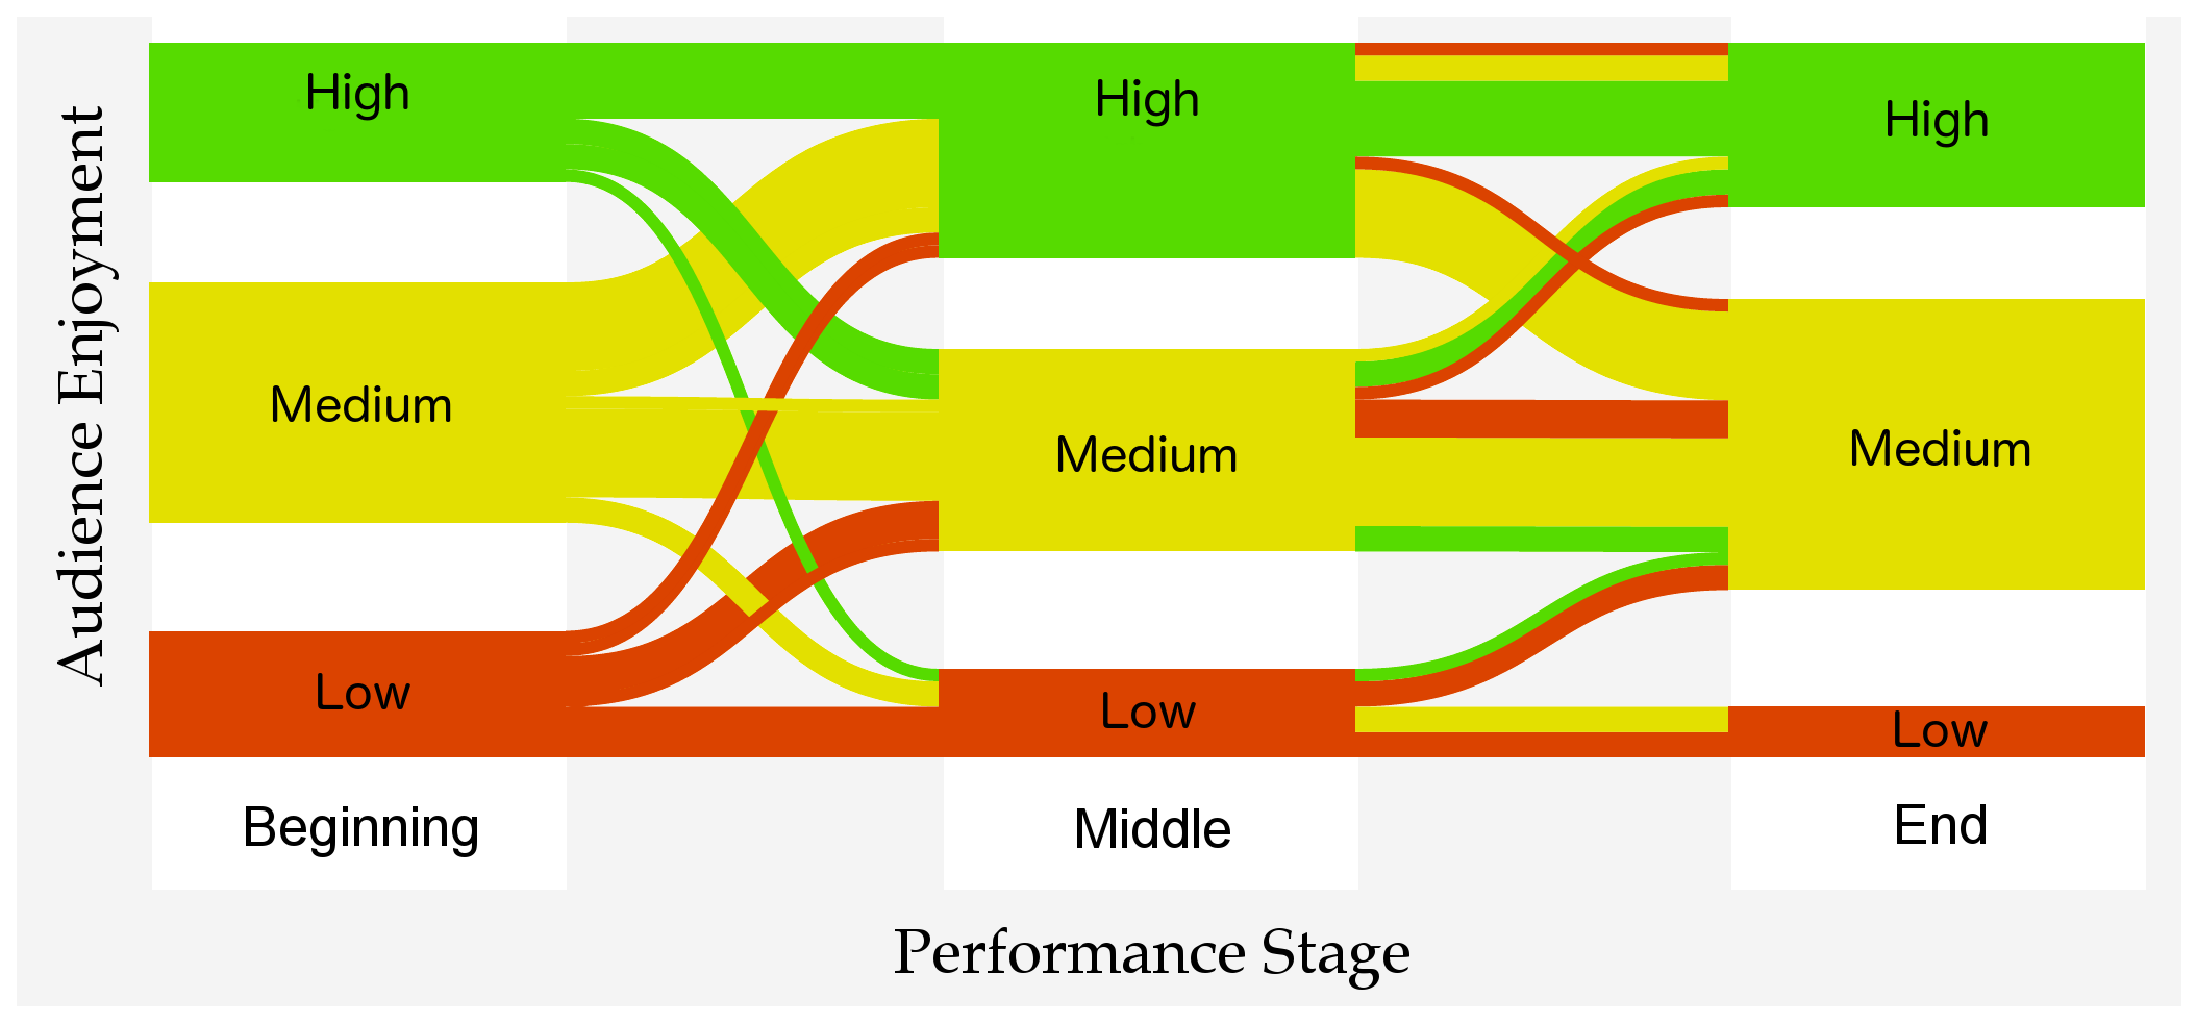
\epsfig{file=didactic-enjoyment-final.eps, width=3.4in}
\caption{Audience reported enjoyment during the beginning, middle and end of the performance with the ``didactic'' condition.}
\label{fig:didactic-enjoyment}
\end{figure}

Overall, a large proportion of the participants stated that both visualisations helped their ``enjoyment" of the performance: $76\%$ stated that the ``aesthetic" visualisations helped their ``enjoyment" and $56\%$ stated that the ``didactic" visualisations helped their ``enjoyment". No significant difference between the visualisation types on ``enjoyment" was found ($\chi^2=3.7733,df=2,p=0.1516$).

Participants were asked to rate their ``enjoyment" during the (self-reported) ``beginning", ``middle" and ``end" of the performances (see Figure~\ref{fig:aesthetic-enjoyment} and Figure~\ref{fig:didactic-enjoyment}). During the ``didactic" performance, $15\%$ of the audience stated that their ``enjoyment" \textit{increased} from the beginning of the performance and was \textit{steady} thereafter. By contrast, $24\%$ of the audience reported this pattern of ``enjoyment" during the ``aesthetic" performance. Approximately $30\%$ of the audience of all (``aesthetic" and ``didactic") performances stated that their enjoyment remained \textit{steady throughout}.

\subsubsection{``Understanding''}

\begin{figure}
\centering
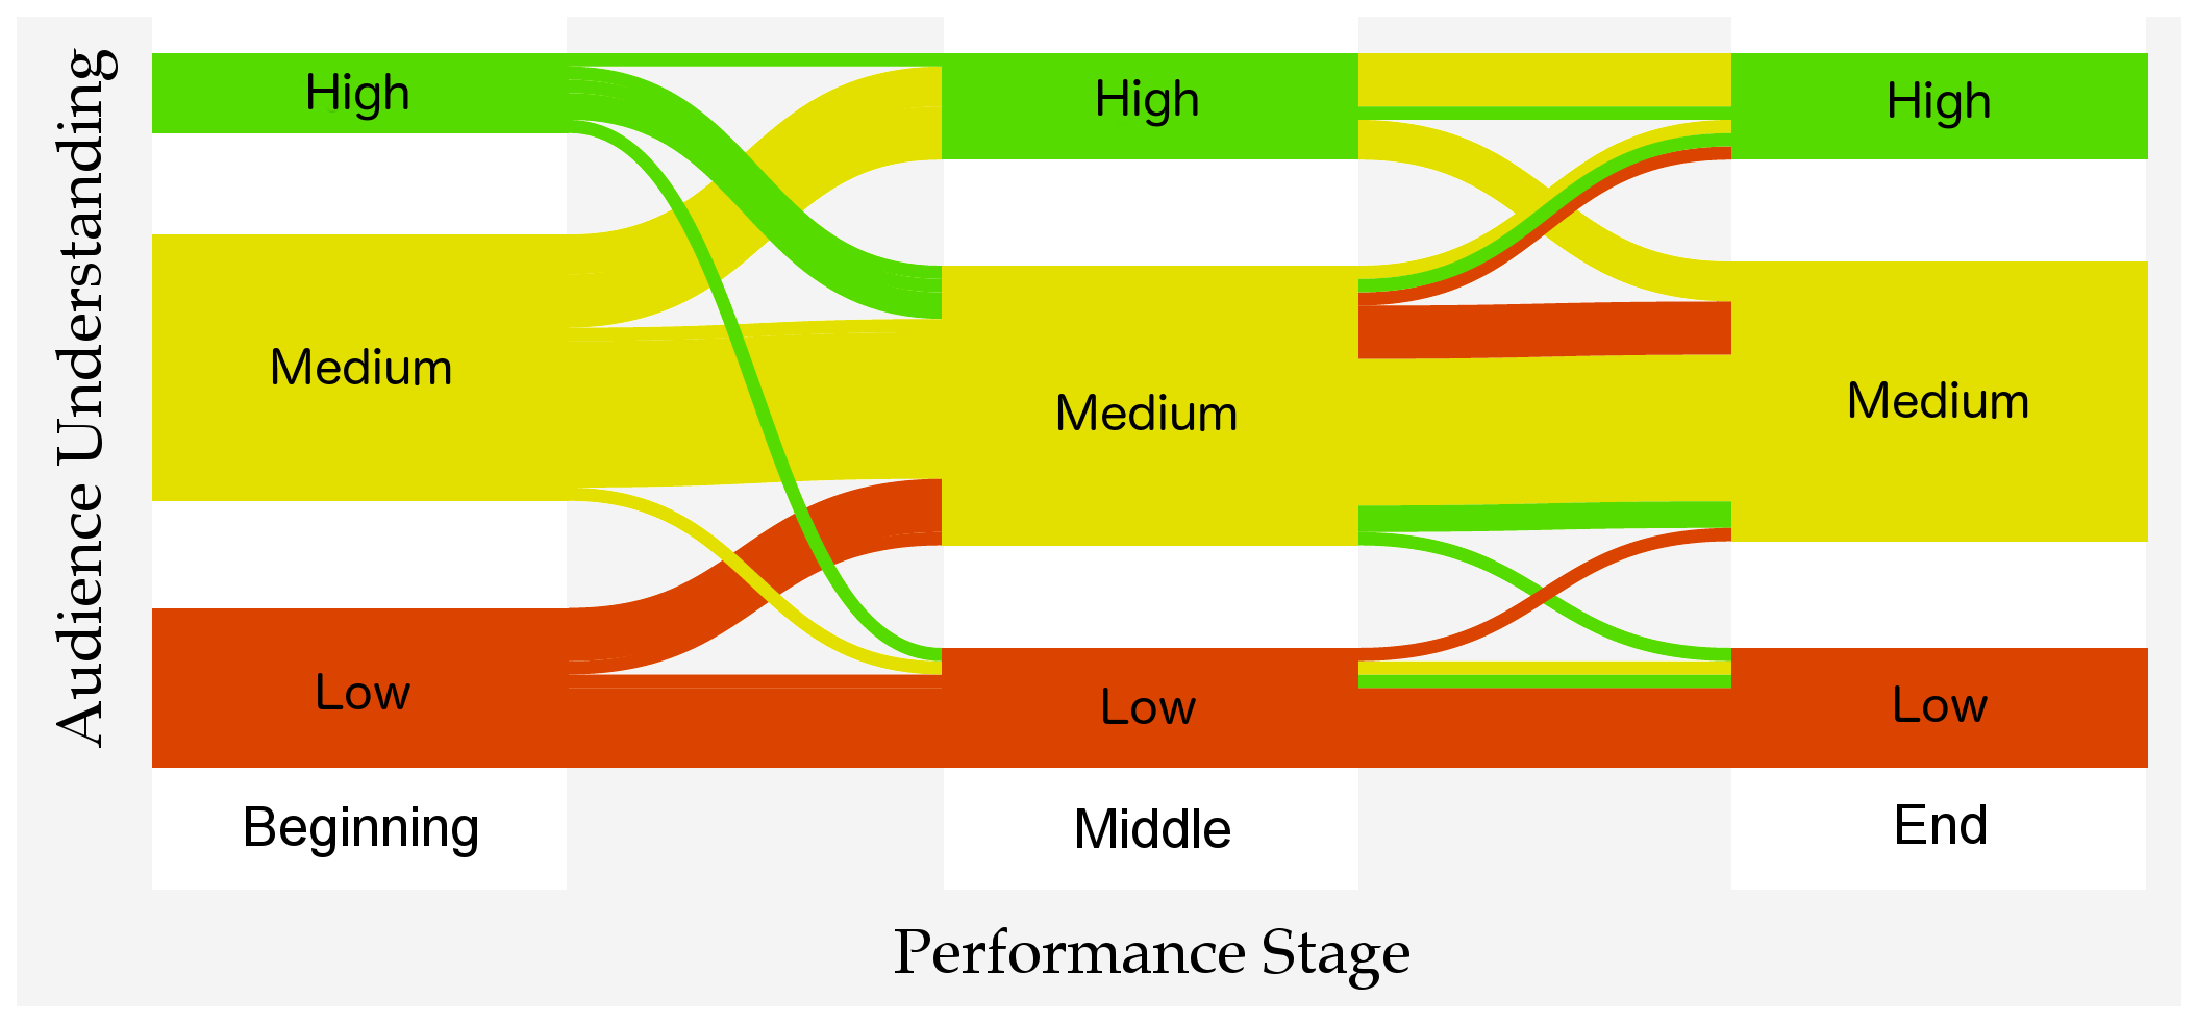
\epsfig{file=aesthetic-understanding-final.eps, width=3.4in}
\caption{Audience reported understanding during the beginning, middle and end of the performance with the ``aesthetic'' condition.}
\label{fig:aesthetic-understanding}
\end{figure}

\begin{figure}
\centering
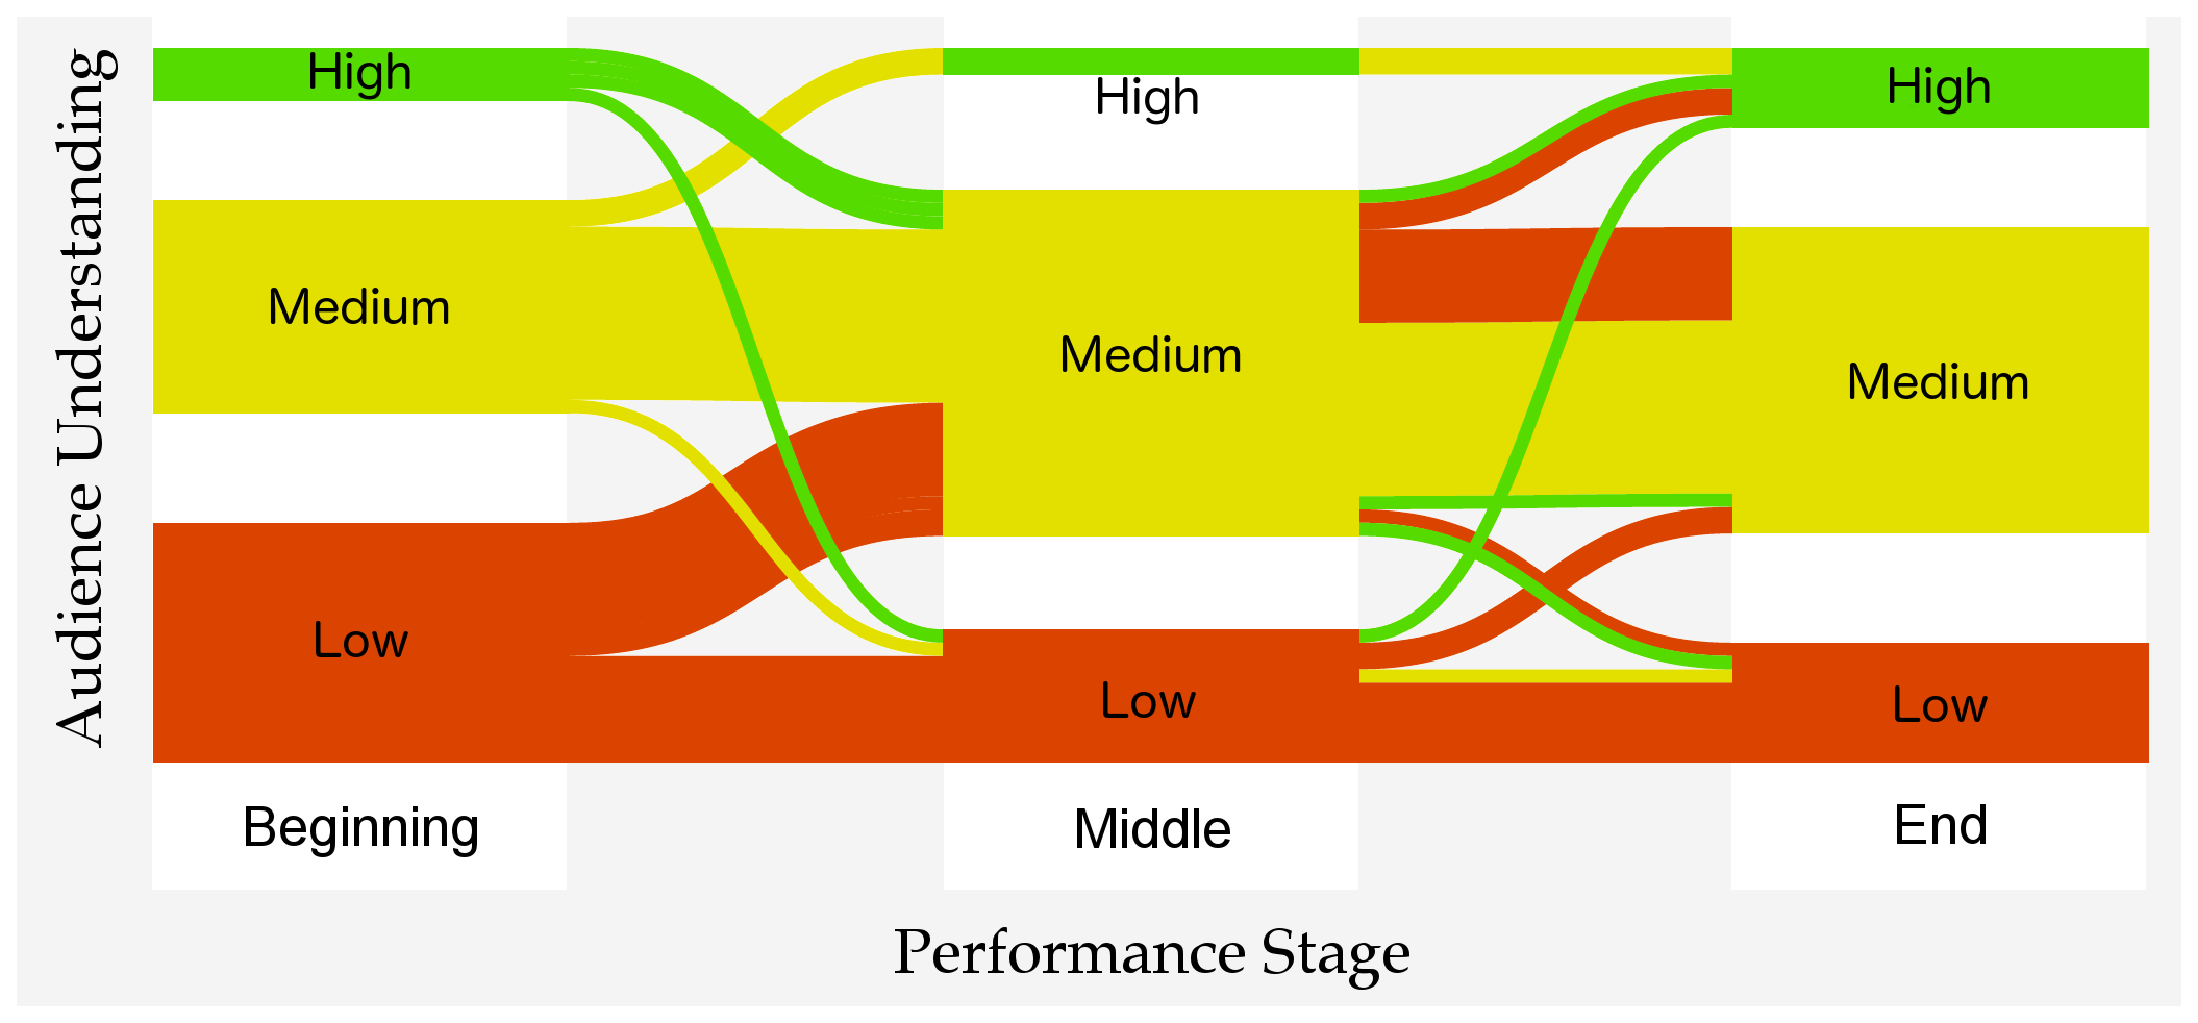
\epsfig{file=didactic-understanding-final.eps, width=3.4in}
\caption{Audience reported understanding during the beginning, middle and end of the performance with the ``didactic'' condition.}
\label{fig:didactic-understanding}
\end{figure}

In response to a specific survey question, $37\%$ of participants stated that, overall, the ``didactic" visualisations \textit{helped them to understand the code} whereas, by contrast, $12\%$ participants stated that, overall, the ``aesthetic" visualisations \textit{helped them to understand the code}. This was a significant difference between these responses ($\chi^2=7.1986,df=2,p=0.02734$).

Participants were asked to rate their ``understanding" during the (self-reported) ``beginning", ``middle" and ``end" of the performance (see Figure~\ref{fig:aesthetic-understanding} and Figure~\ref{fig:didactic-understanding}). During the ``didactic" and ``aesthetic" performances, $49\%$ and $44\%$ of the participants stated, respectively, that their ``understanding" \textit{remained the same} throughout the performances. During the ``didactic" performance, $10\%$ of the audience reported a level of ``understanding" that \textit{trended downwards} (eg. high to low) compared to $20\%$ of the audience during the aesthetic performance. However, this reported advantage of the ``didactic" visualisations was offset by the reported audience ``understanding" at the beginning of the performance where $44\%$ indicated a low ``understanding" with the ``didactic" visualisations compared to only $30\%$ with the ``aesthetic" visualisations. Overall, the figures for ``understanding" are complex and reported levels of ``understanding" fluctuated during the performances. Dramatically, Figure~\ref{fig:didactic-understanding} shows that a very small proportion of the audience reported ``high understanding" during the ``middle" of the performances. One interpretation of this result might be that it took audience members some time to work out what the ``didactic" visualisations were actually showing, and that this conflicted with the first impressions of what some audience members (hence the decrease in levels of ``understanding" from beginning to middle). However, once they finally understood the graphics some audience members were then able to better ``understand" the live-coding performance. 

\subsection{Discussion}

Overall ``enjoyment" of the visualisations was high. This was the case for both the ``aesthetic" and ``didactic" visualisations.
Reported ``enjoyment" of the ``aesthetic" visualisations was higher than for the ``didactic" visualisations but the trends across Figures~\ref{fig:aesthetic-enjoyment} and~\ref{fig:didactic-enjoyment} are complex. 

As discussed above, the small number of ``high" responses for ``understanding" during the ``middle" of the ``didactic" performances, and the decreasing trend from ``high" to ``middle" ``understanding" from ``beginning" to ``middle" of the performances perhaps indicates a higher cognitive load for understanding the ``didactic" visualisations themselves. In fact, features of the ``didactic" visualisation were reported to confuse some members of the audience. One audience member even stated that they ``found them distracting'' and that they ``preferred just to read the code''.

The video-cued-recall interview indicated that the experience of the visualisations of the live coder and the  audience was fundamentally different. Whereas many members of the audience reported that they drifted between focussing on the music, focussing on the visualisations and focussing on the code, the live coder reported that their focus was  purely on the code and the music, rarely drifting. In one particular section of the interview, the live coder stated: ``I definitely wasn't paying attention to them [the visualisations] on the day. In fact I tune them out as best I can because I am just trying to focus on the code''. By contrast, one audience member stated that ``you could see the code being written and the visualisations helped to show when a piece of code started working''. Another audience member stated that ``the visualisations were interesting but distracting''. By contrast, when asked if the visualisations were distracting the live coder stated: ``Ah, no. In general I'm just so focussed on the code''. 

\section{Conclusions}

In the first systematic study of its type, we have identified an opportunity for real-time code visualisations to help improve the audience experience of a live coding computer music performance. With few exceptions, our initial survey of a live coding performance at an arts festival revealed a generally low to medium level of audience ``understanding'' throughout that performance (although almost half the survey respondents indicated a high level of ``enjoyment" throughout).

In an audience experiment, our comparison of two prototype code visualisations indicated that both visualisations seemed to ``help" with ``enjoyment". Significantly more audience members reported that our ``didactic" visualisations ``helped" with ``understanding" but overall trends for both ``enjoyment" and ``understanding" throughout the performances were complex. There are indications of a higher cognitive load for the ``didactic" visualisations than the ``aesthetic" visualisations and this may have influenced audience responses to them. 

In a future extension of this work, design lessons from both visualisation types could be combined together to produce live coding driven visualisations which targeted both the aesthetics as well as a greater understanding of the live coding process. These visualisations could then be compared with the baseline ``no-visualisation" condition in an audience experiment. 

Over 60 years ago, the media theorist Marshall McLuhan stated that ``The business of art is no longer the communication of thoughts or feelings which are to be conceptually ordered, but a direct participation in an experience. The whole tendency of modern communication...is towards participation in a process, rather than apprehension of concepts.'' \cite{McLuhan} Our hope is that future development of the research described in this paper will bring audiences into the \textit{process of live coding} in such a way that they might feel to be active (virtual) collaborators of a highly-skilled live-coding artist.

\bibliographystyle{abbrv}
\bibliography{sigproc}  % sigproc.bib % ACM needs 'a single self-contained file'!

\end{document}
